\documentclass[uplatex,a4j]{jsarticle}
\usepackage[top=35truemm,bottom=30truemm,left=30truemm,right=30truemm]{geometry}
%フォント設定
%\usepackage[deluxe,jis2004]{otf}
\usepackage{amsmath}
\usepackage{amsfonts}
\usepackage{bm}
\usepackage[dvipdfmx]{graphicx}
\usepackage[dvipdfmx]{color}
\usepackage{listings,jlisting}
\usepackage{amsmath,amssymb}
\usepackage{latexsym}
\usepackage{url}
%\usepackage{xcolor}
\usepackage{here}

\providecommand{\tabularnewline}{\\}
\newcommand{\argmax}{\mathop{\rm argmax}\limits}
\newcommand{\argmin}{\mathop{\rm argmin}\limits}

\lstset{
  language=Python,
 	%枠外に行った時の自動改行
 	breaklines = true,
 	%自動改行後のインデント量(デフォルトでは20[pt])
 	breakindent = 10pt,
 	%標準の書体
 	basicstyle = \ttfamily\scriptsize,
 	%コメントの書体
 	commentstyle = {\itshape \color[cmyk]{1,0.4,1,0}},
 	%関数名等の色の設定
 	classoffset = 0,
 	%キーワード(int, ifなど)の書体
 	keywordstyle = {\bfseries \color[cmyk]{0,1,0,0}},
 	%表示する文字の書体
 	stringstyle = {\ttfamily \color[rgb]{0,0,1}},
 	%枠 "t"は上に線を記載, "T"は上に二重線を記載
	%他オプション:leftline,topline,bottomline,lines,single,shadowbox
 	frame = tbrl,
 	%frameまでの間隔(行番号とプログラムの間)
 	framesep = 5pt,
 	%行番号の位置
 	numbers = left,
	%行番号の間隔
 	stepnumber = 1,
	%行番号の書体
 	numberstyle = \tiny,
	%タブの大きさ
 	tabsize = 4,
 	%キャプションの場所("tb"ならば上下両方に記載)
 	captionpos = b
}

\title{新人課題}
\author{津嶋 佑旗}
\date{\today}

\begin{document}
  \maketitle
  \section{配列情報処理}
  \subsection{ヒト21番染色体の先頭コンティグのDNA配列を秋山研サーバから取得し,A/T/G/Cの各塩基数を出力せよ.}
  以下のように実行する.実行環境はPython2で,ghostgw上での動作を確認している.
  \begin{lstlisting}[caption=実行方法, label=run1]
    python 1_1.py /mnt/fs/ohue/newcomer/NT_113952.1.fasta
  \end{lstlisting}
  プログラム本体は以下の通りである.
  \lstinputlisting[caption=1\_1.py, label=program1]{./1_1.py}
  実行した結果が以下の通りである.
  \lstinputlisting[caption=実行結果, label=result1]{./result_1_1.txt}
  
  \subsection{NT\_113952.1.fastaの逆相補鎖を生成するプログラムを作成せよ.}
  以下のように実行する.実行環境はPython2で,ghostgw上での動作を確認している.
  \begin{lstlisting}[caption=実行方法, label=run2]
    python 1_2.py /mnt/fs/ohue/newcomer/NT_113952.1.fasta
  \end{lstlisting}
  プログラム本体は以下の通りである.
  \lstinputlisting[caption=1\_2.py, label=program2]{./1_2.py}
  \lstinputlisting[caption=rev.py, label=programrev]{./rev.py}
  \lstinputlisting[caption=combine.py, label=programcombine]{./combine.py}
  実行結果はresult\_1\_2.txtとして別添する.
  
  \subsection{ウィンドウ幅$w$,ステップ幅$s$で,ウィンドウ内のGC含量を出力するプログラムを作成し,NT\_113952.1.fastaに$w=1000$,$s=300$で適用した結果をgnuplot等Excel以外のツールでプロットせよ.}
  以下のように実行する.実行環境はPython2で,ghostgw上での動作を確認している.
  \begin{lstlisting}[caption=実行方法, label=run3]
    python 1_3.py /mnt/fs/ohue/newcomer/NT_113952.1.fasta 1000 300 > data.txt
  \end{lstlisting}
  プログラム本体は以下の通りである.また,\ref{programcombine}も使用する.
  \lstinputlisting[caption=1\_3.py, label=program3]{./1_3.py}
  実行結果をgnuplotで描画した結果以下のようになった.
  \begin{figure}[htbp]
    \begin{center}
      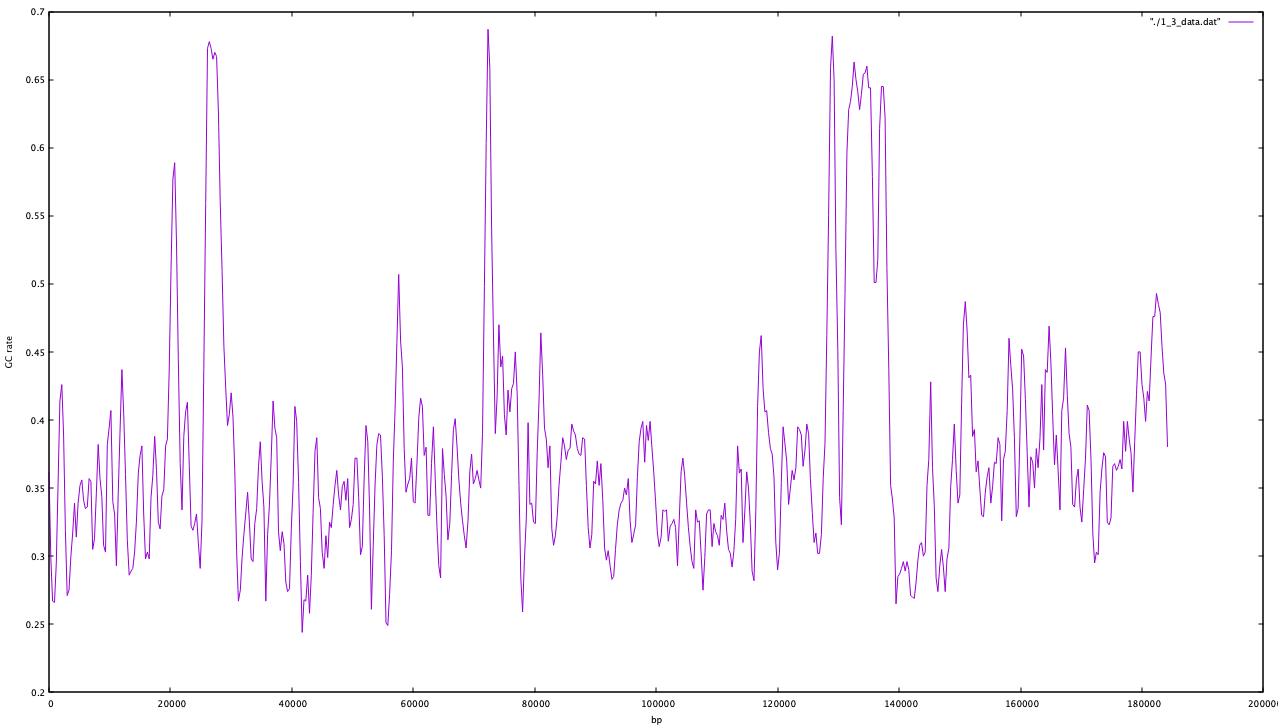
\includegraphics[width=15cm]{1_3_plot.png}
      \caption{グラフ}
    \end{center}
  \end{figure}
  
  \subsection{引数で与えられた部分配列を検索し,何文字目に現れたかを表示するプログラムを作成せよ(逆相補鎖上も検索すること).部分配列をGAATTCおよびATGとし,NT\_113952.1.fastaに適用せよ.}
  以下のように実行する.実行環境はPython2で,ghostgw上での動作を確認している.
  \begin{lstlisting}[caption=実行方法, label=run4]
    python 1_4.py /mnt/fs/ohue/newcomer/NT_113952.1.fasta GAATTC
    python 1_4.py /mnt/fs/ohue/newcomer/NT_113952.1.fasta ATG
  \end{lstlisting}
  プログラム本体は以下の通りである.また,\ref{programrev}と\ref{programcombine}も使用する.
  \lstinputlisting[caption=1\_4.py, label=program4]{./1_4.py}
  \lstinputlisting[caption=findall.py, label=programfindall]{./findall.py}
  実行した結果が以下の通りである.ただし,ATGの結果については極端に長いためresult\_1\_4\_ATG.txtとして別添する。
  \lstinputlisting[caption=実行結果(GAATTC), label=result4]{./result_1_4_GAATTC.txt}
  
  \subsection{NT\_113952.1.fastaを6つの読み枠でアミノ酸配列に変換せよ.Stopコドンはアンダースコアで表示すること.}
  以下のように実行する.実行環境はPython2で,ghostgw上での動作を確認している.
  \begin{lstlisting}[caption=実行方法, label=run5]
    python 1_5.py /mnt/fs/ohue/newcomer/NT_113952.1.fasta
  \end{lstlisting}
  プログラム本体は以下の通りである.また,\ref{programrev}と\ref{programcombine}も使用する.
  \lstinputlisting[caption=1\_5.py, label=program5]{./1_5.py}
  \lstinputlisting[caption=decode.py, label=programdecode]{./decode.py}
  
  \section{タンパク質構造情報処理}
  \subsection{PyMOLソフトウェアを利用し,ヒトのヘモグロビンの構造をチェインごとに異なる色で表示し,4量体であることを確認せよ。また,Aチェインだけを表示し,タンパク質鎖をcartoon表示して2次構造に従って色付けし,結合するヘムをstick表示して原子ごとに色分けせよ。}
  チェインごとに色分けしたヘモグロビンが画像\ref{2_6_1}である。
  \begin{figure}[H]
    \begin{center}
      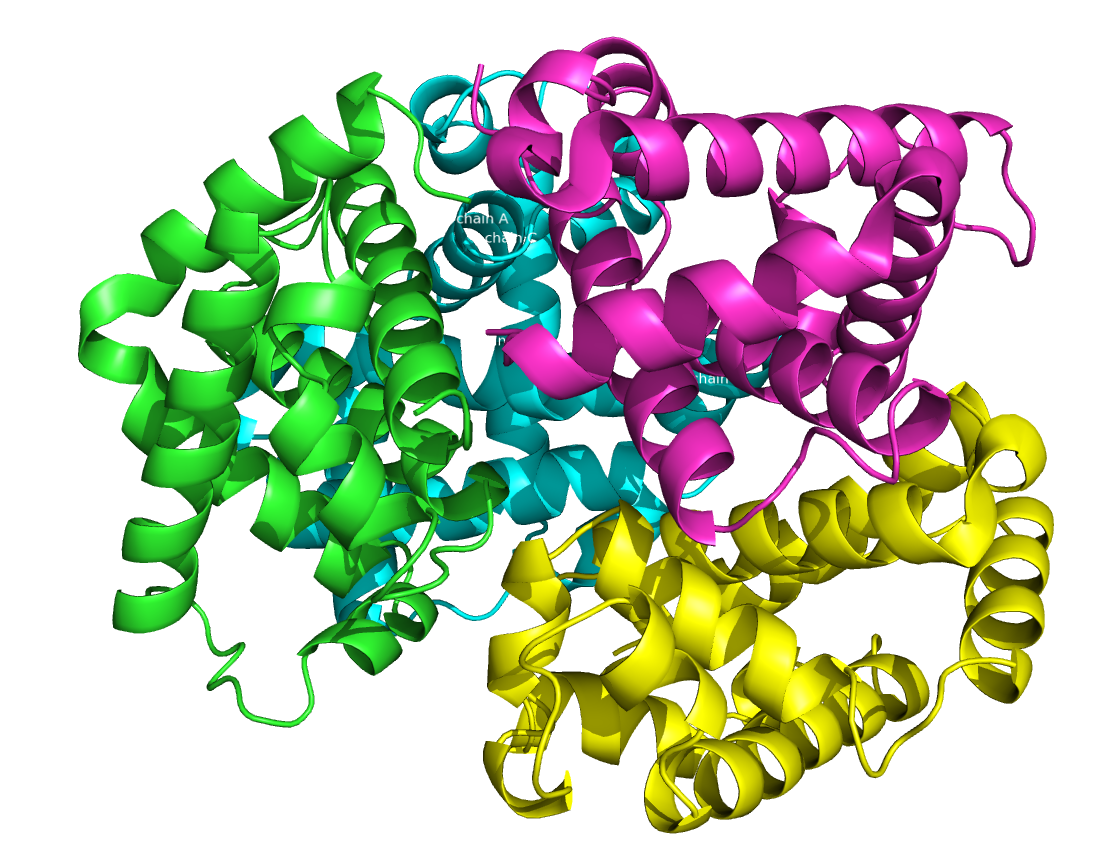
\includegraphics[width=12cm]{1BUW.png}
      \caption{ヘモグロビン}
      \label{2_6_1}
    \end{center}
  \end{figure}
  また,Aチェインとヘムを表示したものが画像\ref{2_6_2}である。
  \begin{figure}[H]
    \begin{center}
      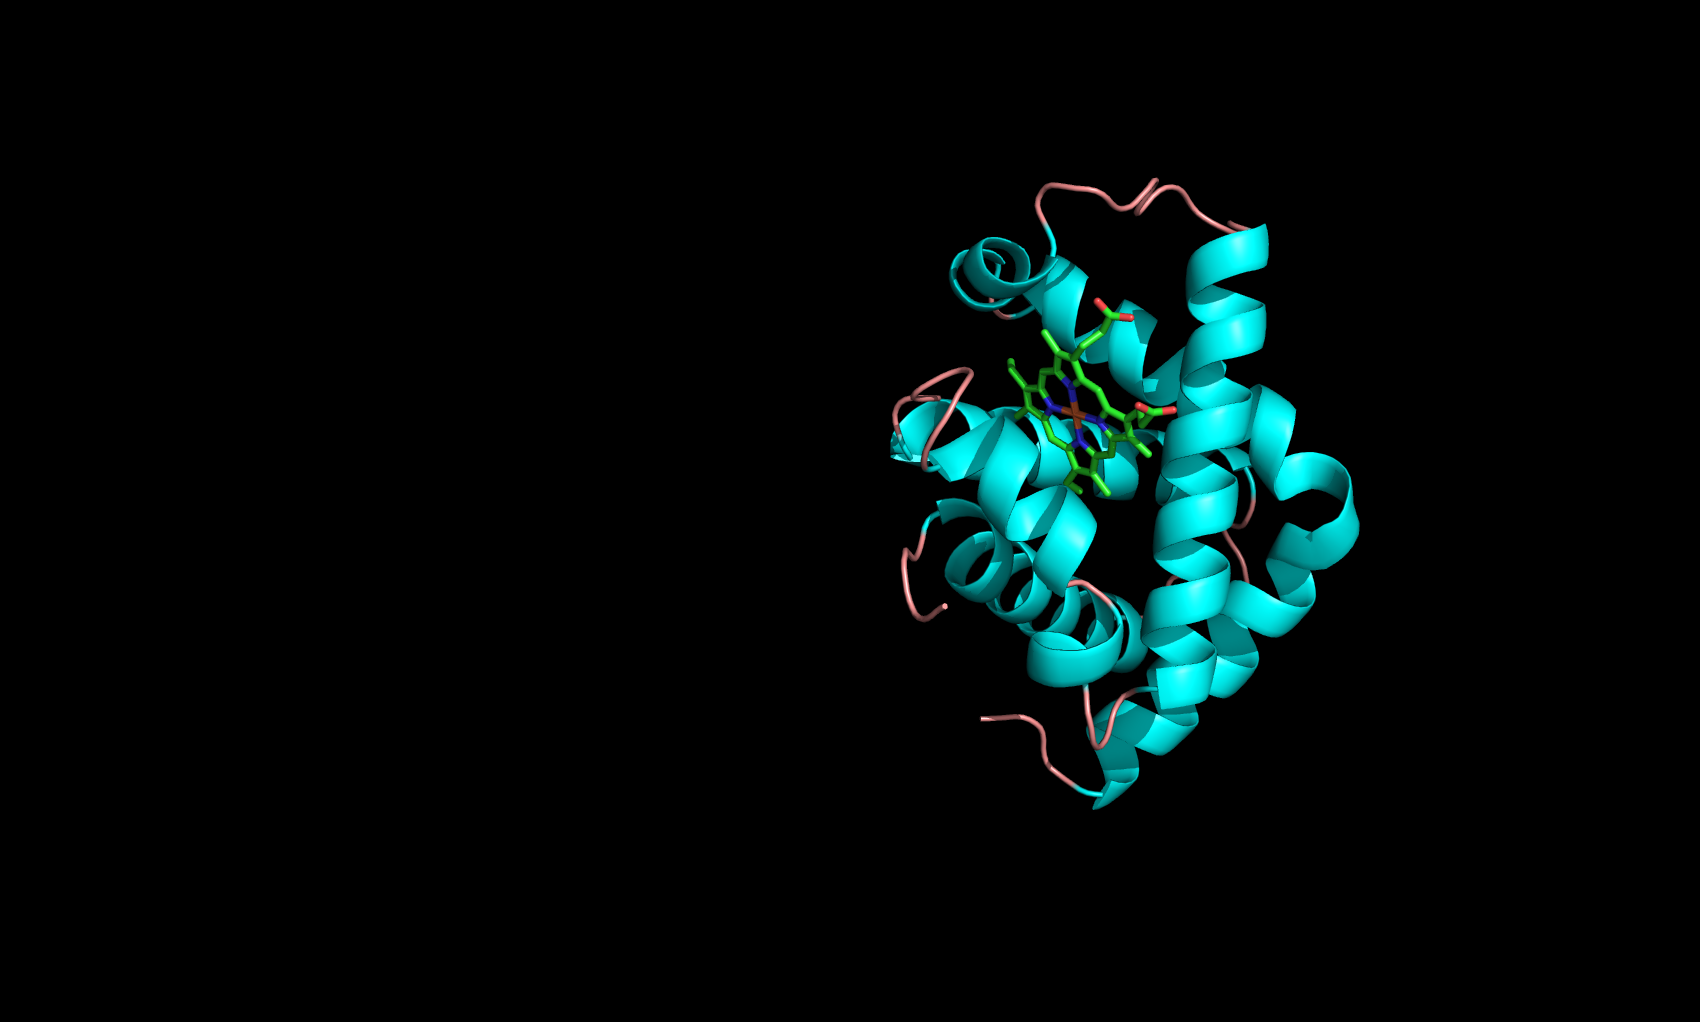
\includegraphics[width=12cm]{hem.png}
      \caption{Aチェインとヘム}
      \label{2_6_2}
    \end{center}
  \end{figure}
  
  \subsection{PDBファイル名とチェイン名を引数にして、その回転半径を計算するプログラムを作成せよ。}
  以下のプログラムを作成した。実行環境はAnaconda2のPython 2.7環境である。
  \lstinputlisting[caption=2\_7.py, label=program6]{./2_7.py}
  このプログラムを次のように実行する。
  \begin{lstlisting}[caption=実行方法, label=run6]
    python 2_7.py ./1BUW.pdb A
  \end{lstlisting}
  結果は次の通りである。
  
  \subsection{上記のプログラムの結果を利用し、PyMOLで重心から回転半径の範囲内にある原子を赤で、範囲外にある原子を青で色付けせよ。}
  
  \section{機械学習}
  \subsection{Pythonのscikit-learnのSVMでionosphereのデータの10-fold Cross Validationを実施せよ。予測性能としてprecision、recall、MCC、ROC曲線のAUC値(AUROC)、F-scoreを求めよ。カーネルはRBFカーネルとし、パラメータは適宜定めよ。}
  
  \subsection{ionosphereデータにおいて、より良いRBFカーネルパラメータ$\gamma$とコストパラメータ$C$の値を探索せよ。評価方法は10-fold Cross Validationとし、評価基準はAUROCとF-scoreの2通りを試すこと。}
  
\end{document}
